%% AMS-LaTeX Created by Wolfram Mathematica 7.0 : www.wolfram.com

\documentclass{article}
\usepackage{amsmath, amssymb, graphics}

\newcommand{\mathsym}[1]{{}}
\newcommand{\unicode}{{}}

\begin{document}

\noindent\(\pmb{\text{Z1}[\text{s$\_$}]\text{:=}\frac{\text{Gamma}\left[-\frac{s}{2}\right]}{2\text{Gamma}[-s]}\text{Hypergeometric1F1}\left[-s,\frac{1}{2},\frac{1}{4}\right]}\)

\noindent\(\pmb{\text{Plot}\left[\frac{\text{Gamma}\left[-\frac{s}{2}\right]}{2\text{Gamma}[-s]}\text{Hypergeometric1F1}\left[-s,\frac{1}{2},\frac{1}{4}\right],\{s,0,5.1\},\text{AxesOrigin}\to
\{0,0\}\right]}\)

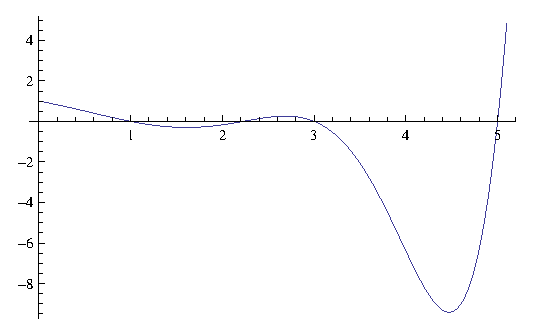
\includegraphics{PlotsRiemannH_gr1.eps}

\noindent\(\pmb{\text{Plot}\left[\text{Abs}\left[\text{Z1}\left[-\frac{1}{4}+i*t\right]\right],\{t,0,100\},\text{AxesOrigin}\to \{0,0\}\right]}\)

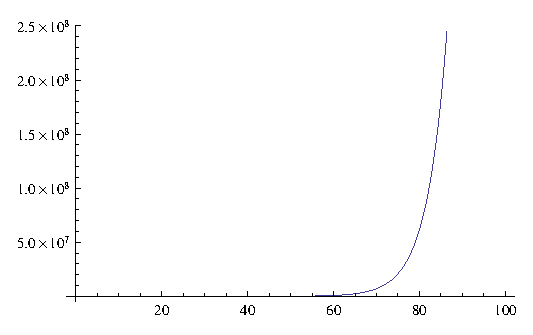
\includegraphics{PlotsRiemannH_gr2.eps}

\end{document}
